The primary variables tested in this experiment were the efficacy of the merging algorithms at removing redundancy and the efficency of these algorithms.

\subsection{Removal Efficacy}
The algorithm combinations' results were varied.
The top performing algorithm was the custom made algorithm combined with hierarchical clustering, which outperformed all others by a significant margin.

\begin{figure}
	\begin{center}
	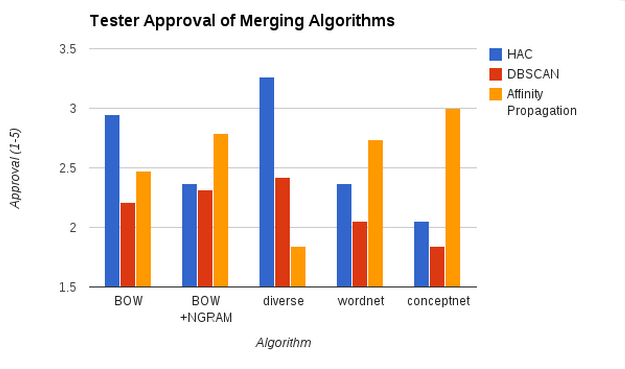
\includegraphics[width=0.75\textwidth]{figures/ratechart.png}
	\caption{The user approval of various methods.}
	\label{fig:approv}
	\end{center}
\end{figure}

An f-test of the results indicated that there was significant difference between the answer received ($F \le 0.05$) !!does this work?!!.  A secondary T-test between the highest custom algorithm and the second-highest yielded a significant difference as well ($p < 0.05$). This shows strong evidence that the custom algorithm performed the best of all the algorithms.

The results also showed, interestingly, that the bag of words algorithm performed very well when utilized with the hierarchical aggomerative clustering, performed second best.
This seems to indicate that although simple bag-of-words was not an effective form of sentence comparison, in the right situations, it can be utilized as an effective means of classifying sentences (at the very least, for human evaluation).
Figure \ref{fig:approv} illustrates the results. 
Note that in this chart, the custom algorithm is labeled as ``diverse'' in reference to its usage of components from a diverse assortment of algorithms.

\subsection{Runtime analysis}

The runtime of each algorithm was also evaluated.
the bag of words and n-grams only models performed very well, and were able to finish in significantly less time than the other algorithms.
\begin{figure}
	\begin{center}
	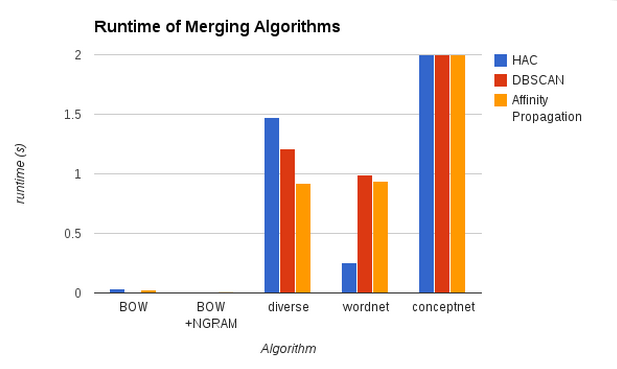
\includegraphics[width=0.75\textwidth]{figures/rtchart.png}
	\caption{The runtime of various algorithms. Note that the conceptnet time was so large that the bar had to be truncated for this graph.}
	\label{fig:s}
	\end{center}
\end{figure}

The custom diverse algorithm performed slower than the other algorithms tested, though this result may not necessarily scale with the size of the matrix. 
The most efficient algorithms for agglomerative clustering run in $O(n^2)$ time, and this is not extensively impacted by the additional computation to compute wordnet similarity.
At most it can be increased to $O(n^2T)$, where T is the distance to the nearest common ancestory in the wordnet hierarchy between two terms. !!!is n3 time still efficient?!!

Further, affinity propagation, which operates slower than hierarchical clustering, was shown to actually be quicker.
Most likely, the data used in this experiment was not large enough to accurately gage the runtime of these algorithms.

One efficiency that was sufficiently measured, however, was that of the conceptnet algorithm.
The full conceptnet was too large to be deployed onto a small webapp server (it is approximately 5gb in size). 
Thus, for this experiment, the rest api was utilized. 
The latency from the http requests necessary to compute the distance between two terms, combined with the server side computation of this task, led the conceptnet runtime to be much larger than any of the other methods.
Figure \ref{fig:approv} illustrates the results.
%interface
%success with interface
%better than normal
%vast, irreconcilable differences
	% john's example
%able to finish in good time for all examples
%better reviews than solo
%observations- users are able to compromise on an end
%users generally go find optimal- they all rate highly 

%ai
%timing results (not importatn)
%accuracy
	%f test shows at least one is better
	%the top is significantly better than next, so it means that it is better
